\documentclass{standalone}
\begin{document}
	\chapter{Ground Glass Identification Pipeline}
	
	Since the end of 2019, COVID-19 has widely spread all over the world. Up to now the gold standard for the identification of the pathology is the 
	RT-PCR even if it is reported that its sensitivity might not be enough for COVID-19 identifications~\cite{ART:Ai} and requires a lot of time to provide results.\\Has been observed that  several chest CT scans collected from COVID-19 patients shown bilateral patchy shadows or ground glass opacity (GGO) in the lung~\cite{ART:Ai}~\cite{ART:Wang}, which makes interesting tp investigates this technique to help diagnosis, monitoring the course of the disease and check the recovery of healed patients, since the GGO pattern may change according to the state of the disease~\cite{ART:Bernheim}.
	Austin in Glossary of terms for CT of the lungs~\cite{ART:Austin} define the Ground Glass Opacities as hazy increased attenuation of lung, with 
	preservation of bronchial and vascular margins caused by partial filling of air spaces, interstitial thickening, partial collapse of alveoli, normal expiration, or increased capillary blood volume. This kind of lesion is not exclusive of COVID-19 but can be associated to many other disorders like edema, bacteria infection or alveolar haemorrhage.  
	However the study of the particular patterni in combination with other techniques may help early diagnosis of this pathology and the monitoring of the recovery, has shown by ~\cite{ART:Bernheim}, since the GGO pattern and the involving of lung parenchima changes according to the severity of the disesase and the recovery stage.\\
	
	So becomes very important to identify this kind of lesions for the reasons given before. Up to know the identification of these lesions is made mainly by manual or semi-automatic segmentation, both of them are time consuming, error prone and subjective, since require the interaction of specialized operators. To overcome this issues an automatic way to obtain these information is desirable, since allows to obtain measures that do not depend n operator subjectivity; moreover it is desirable to obtain segmentation results in a small amount of time, which is not compatible with manual or semi-automatic segmentation.\\
	
	In this chapter I will describe in details the implementation of a segmentation pipeline which allows a fast and automatic segmentation of GGO. 
	
		 
	
	\begin{figure}[h!]\label{fig:HealthVSCovid}
		\centering
		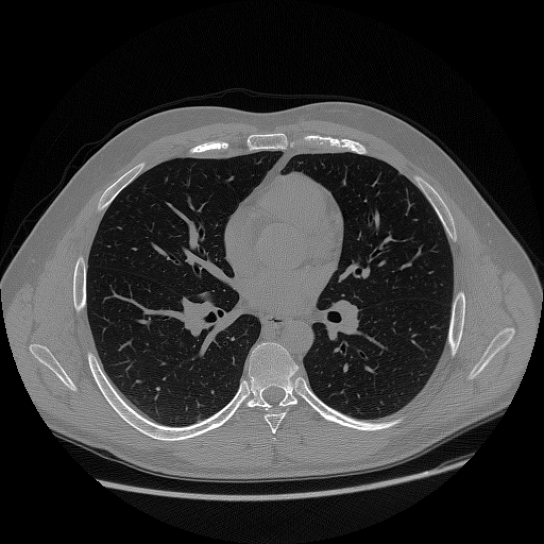
\includegraphics[scale=.5]{healthy.png}
		\quad
		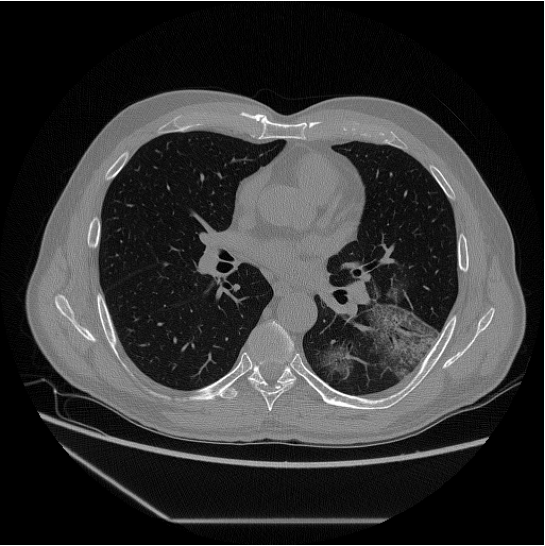
\includegraphics[scale=.5]{ggo.png}
		\caption{CT scan of thorax for an healthy patient(left) and a COVID-19 affected one(right) in which we can observe a huge amount of GGO in the right lung}
	\end{figure} 
	
	
\end{document}